\subsection{Design Evolution}
The development of \textbf{Kamikaze} was the result of a step-by-step design process that began with a critical evaluation of last year’s model, Shiro Kaijin (Figure \ref{fig:shiro_kaijin}). By identifying its limitations, we carefully assessed alternative solutions, ensuring that each design decision balanced performance, cost, and operational efficiency. 

\begin{figure}[h]
    \centering
    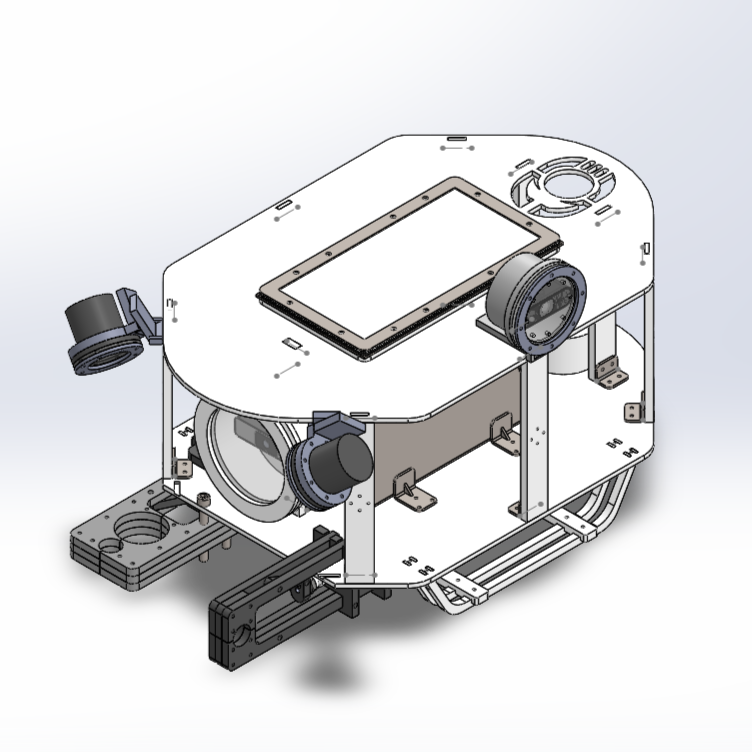
\includegraphics[width=0.7\columnwidth]{Sections/2Design Rationale/images/Shiro Kaijin.png}
    \caption{Last year's ROV - Shiro Kaijin.}
    \label{fig:shiro_kaijin}
\end{figure}

Our team conducted structured brainstorming sessions to explore innovations that would enhance functionality while maintaining cost-effectiveness. Through a holistic systems approach, we ensured seamless integration between mechanical, electrical, and software components, optimizing overall performance. As a result, Kamikaze (Figure \ref{fig:Kamikaze}) represents a well-planned evolution that enhances reliability, efficiency, and mission adaptability.

\begin{figure}[hb!]
    \centering
    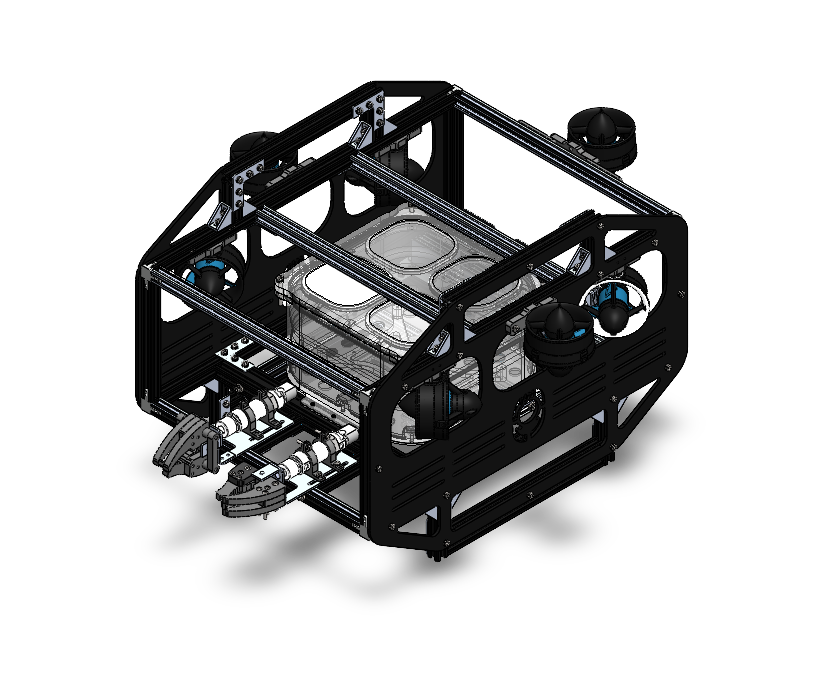
\includegraphics[width=0.7\columnwidth]{Sections/2Design Rationale/images/Kamikaze.png}
    \caption{Kamikaze.}
    \label{fig:Kamikaze}
\end{figure}

\subsubsection{Mechanical System Evolution}
\vspace{0pt}
\textbf{Frame and Structural Improvements}

Shiro Kaijin’s frame was constructed entirely from HDPE, which posed challenges in component fixation. Drilling holes for mounting often led to overlap issues, making modifications difficult. To address this, Kamikaze features a modular aluminum extrusion body, enabling flexible component placement, quick adjustments, and easier repairs.

\vspace{0.2cm}
\textbf{Canister Evolution}

One of the major design advancements in Kamikaze is the transition from an aluminum canister to a 3D-printed PETG canister. While aluminum provided durability, it was costly, difficult to modify, and unnecessarily heavy. The new 3D-printed PETG canister offers greater design flexibility, allowing for customized internal layouts, easy adjustments, and rapid prototyping without the constraints of metal fabrication.

\vspace{0.2cm}
\textbf{Propulsion System}

Kamikaze improves upon its predecessor’s six-thruster configuration by adopting a seven-thruster setup, enhancing maneuverability and control. However, in line with cost-efficiency objectives, all thrusters from last year’s model were reused, maintaining a balance between improved functionality and resource optimization.

\vspace{0.2cm}
\textbf{Gripper Mechanism Enhancement}

Shiro Kaijin’s gripper was limited to fixed circular openings, restricting it to predefined object sizes. Kamikaze introduces a versatile gripping mechanism capable of adapting to various object dimensions, significantly increasing efficiency and flexibility in underwater tasks.

\vspace{0.2cm}
\textbf{Improved Piloting and Camera System}

Kamikaze enhances operational efficiency with an upgraded camera system supporting multiple camera types with rotation and tilt functionality. This ensures a comprehensive, adaptable view of the environment, improving pilot control and situational awareness.

\subsubsection{Electrical System Evolution}

\textbf{Power Connection and Cable Management Issues}

Shiro Kaijin faced instability in power connections due to disorganized cables, causing electrical noise and intermittent connectivity. Each ESC was connected separately, leading to excessive wiring and limited space within the canister. To resolve this, Kamikaze integrates all ESCs into a single PCB, significantly reducing cable clutter, minimizing electrical noise, and improving system stability. Additionally, an STM32 microcontroller was added to the power PCB, further optimizing wiring and ensuring a more reliable electrical system.

\vspace{0.2cm}
\textbf{Inadequacy of Arduino UNO}

The Arduino UNO, used as the main controller, struggled to handle multiple sensors, leading to irregular data handling and performance issues. Kamikaze replaces it with an STM32 microcontroller, offering better stability, higher processing power, and improved efficiency for industrial applications. To further enhance system communication, a CAN bus was integrated, enabling reliable data exchange between multiple STM32s, reducing wiring complexity, and allowing independent node resets without affecting the overall system.

\vspace{0.2cm}
\textbf{Limitations of MS5540 Depth Sensor}

The MS5540 depth sensor was inaccurate, slow, and costly, making it an inefficient choice. Kamikaze replaces it with a custom-designed depth sensor, providing real-time, accurate measurements and better connectivity options. To improve monitoring capabilities, voltage and current sensors were also implemented, allowing precise tracking of power consumption and early detection of system faults.

\vspace{0.2cm}
\textbf{Reliability of Main Control PCB}

Shiro Kaijin used relays in the main control PCB, which affected system stability. Kamikaze replaces them with MOSFETs, enhancing reliability and improving overall performance. Additionally, a debugging node using the W5500 Ethernet module was introduced, enabling real-time system monitoring and remote reset of multiple nodes, ensuring continuous stability and efficient troubleshooting.

\vspace{0.2cm}
\textbf{Switching from Copper to Aluminum Wires}

Copper wires in high-power transmission corroded quickly, posing safety risks. Kamikaze replaces them with aluminum wires, which are lighter, more durable, and resistant to redox reactions, ensuring safer and more efficient power transmission.

\subsubsection{Software System Evolution}

Something about the software system evolution. \lipsum[1]

\begin{figure}[h]
    \centering
    \rule{0.8\columnwidth}{4cm}
    \caption{Software System Evolution.}
    \label{fig:software_system}
\end{figure}